\documentclass[problem]{mcs}

\begin{pcomments}
  \pcomment{FP_product_rule_and_independence}
  \pcomment{by Mike Mekonnen 12/3/11}
\end{pcomments}

\pkeywords{
  product_rule
  independence
}

%%%%%%%%%%%%%%%%%%%%%%%%%%%%%%%%%%%%%%%%%%%%%%%%%%%%%%%%%%%%%%%%%%%%%
% Problem starts here
%%%%%%%%%%%%%%%%%%%%%%%%%%%%%%%%%%%%%%%%%%%%%%%%%%%%%%%%%%%%%%%%%%%%%

% F11

\begin{problem}
Construct a probability space $\sspace$ such that $\sspace$ contains
three events $A$, $B$, and $C$ with the following properties:

\begin{itemize}
\item The three events satisfy the ``\idx{product rule}.''  That is,
\[
\pr{A \cap B \cap C} = \pr{A} \cdot \pr{B} \cdot \pr{C}.
\]

%\item No two out of the three events satisfy the product rule.

\item The events are \emph{not} \idx{mutually independent}.
\end{itemize}

\hint It may be helpful to draw a \idx{Venn diagram} for $\sspace$
containing the three events, and then incrementally fill in the
probabilities of the disjoint regions.

\begin{solution}
One possible answer can be constructed as follows: in the Venn diagram
shown below,
\begin{align*}
\pr{A}  = \pr{B} = \pr{C}  & = x + y\\
\pr{A \cap B} = \pr{A \cap C} = \pr{B \cap C} &  = y\\
\pr{A \cap B \cap C} & = y
\end{align*}


\begin{figure}[h]
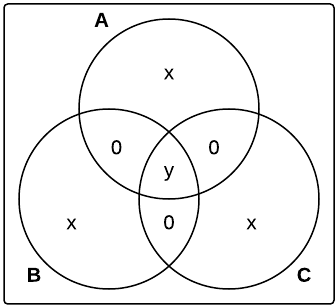
\includegraphics[height=2in]{product-rule-independence-venn}
\end{figure}


With this setup, we need to find $x$ and $y$ such that,
\begin{align*}
\pr{A \cap B \cap C} & = y = (x+y)^3 = \pr{A} \cdot \pr{B} \cdot \pr{C}\\
\pr{A \cap B} & = y \neq (x+y)^2 = \pr{A} \cdot \pr{B}\\
\pr{A} + \pr{B} + \pr{C} & = 3x+y \le 1.
\end{align*}
Take
\[
y = \frac{1}{27}.
\]
From $(x+y)^3 = y$, we get that
\[
x = \frac{8}{27}.
\]
The second requirement is satisfied since $(x+y)^2 = \frac{1}{9}$, which is
different from $y$.  The third requirement is also satisfied since
$3x+y = \frac{25}{27} < 1$.

\end{solution}

\end{problem}

%%%%%%%%%%%%%%%%%%%%%%%%%%%%%%%%%%%%%%%%%%%%%%%%%%%%%%%%%%%%%%%%%%%%%
% Problem ends here
%%%%%%%%%%%%%%%%%%%%%%%%%%%%%%%%%%%%%%%%%%%%%%%%%%%%%%%%%%%%%%%%%%%%%

\endinput
